%%%%%%%%%%%%%%%%%%%%%% PREAMBULE %%%%%%%%%%%%%%%%%%%%%%%%%%%%%%%%%%%%%%%%

%%%%%%%%%%%%%%%% PARAMETRES DU DOCUMENT %%%%%%%%%%%%%%%%%%%%%%%%%%%%%%%%%
\documentclass[12pt,a4paper]{article}
\usepackage[utf8]{inputenc}
\usepackage[T1]{fontenc}
\usepackage[french]{babel}

%%%%%%%%%%%%%%%%%%%%% PACKAGES %%%%%%%%%%%%%%%%%%%%%%%%%%%%%%%%%%%%%%%%%%
\usepackage{hyperref}
\usepackage{shorttoc}
\setlength{\parindent}{0pt}
\usepackage[top=2cm,bottom=2cm,right=2cm,left=2cm]{geometry}
\usepackage{multicol}
\usepackage{nccrules}
\usepackage{eurosym}
\usepackage{listings}
\usepackage{caption}
\usepackage{makecell}
\usepackage{graphicx}
\usepackage{subfigure}
\usepackage{hyperref}
\usepackage{biblatex}
\addbibresource{biblio.bib}

%%%%%%%%%%%%%%%%%%%%%%%%%%%%%%%%%%%%%%%%%%%%%%%%%%%%%%%%%%%%%%%%%%%%%%%%%


%%%%%%%%%%%%%%% PARAMETRAGES PACKAGES %%%%%%%%%%%%%%%%%%%%%%%%%%%%%%%%%%%
\captionsetup{labelformat=empty}

\hypersetup{
	colorlinks=true,
	linkcolor=blue,
	urlcolor=blue,
	citecolor=black
	}

%%%%%%%%%%%%%%%%%%%%%%%%%%%%%%%%%%%%%%%%%%%%%%%%%%%%%%%%%%%%%%%%%%%%%%%%%

\setlength{\fboxrule}{.2pt}

%%%%% PAGE DE TITRE %%%%
\title{Groupe 3 - Synthèse}

\author{Hugo Ligneres - Samantha Ortega - Hamza Takarrouht - Hugo Rytlewski}

\date{UE L313 - Semaine 4}

\begin{document}

\maketitle

\hrulefill
\vspace{6cm}
\begin{center}
	
\includegraphics[scale=.4]{../images/univ.png}
		\\
		\vspace{2cm}
	
\includegraphics[scale=.25]{../images/cvtic.png}
\end{center}

%%%%%%%%%%%%%%%%%%%%%%%%%%%%%%%%%%%%%%%%%%%%%%%%%%%%%%%%%%%%%%%%%%%%%%%%%%
\newpage

\tableofcontents

\newpage

\section{Introduction}

Pour cette deuxième et dernière semaine des projets de groupe, nous devions réaliser un clone de Watson, cette fois-ci avec le framework Symfony et les différents outils associés. Le but était de mettre en place un système similaire à celui de Watson, c'est-à-dire un CRUD permettant de gérer le stockage et l'affichage des liens sur le site. \\

Nous allons d'abord voir comment nous nous sommes organisés pour ce travail de groupe. Puis, dans une deuxième partie, nous reviendrons sur ce que nous avons produit.

\section{Organisation générale}

	\subsection{Répartition du travail}
	
	
Dès le début de la semaine, nous avons défini une répartion du travail pour être le plus efficace possible. Chaque membre avait des responsabilités différentes :


\begin{table}[!h]
	\centering
		\begin{tabular}{|c|l|}
			\hline
			& \\
			Nom & Mission \\ 
			& \\\hline
			& \\
			Hugo L & \makecell[l]{Installation du projet \\ Gestion dépôt GitHub \\ Rédaction du rapport de synthèse \\ Rendu Twig/CSS}\\ 
			& \\ \hline
			& \\
			Samantha & \makecell[l]{Formulaire de l'ajout de liens \\ Rendu Twig/CSS} \\ 
			& \\ \hline
			& \\
			Hamza & \makecell[l]{Pagination \\ Amélioration de la suppression }\\ 
			& \\ \hline
			& \\
			Hugo R & Mise en place du CRUD \\ 
			& \\ \hline
		\end{tabular}
	\caption{Répartition des rôles au sein du groupe}
\end{table}	

\newpage
		
	\subsection{Méthode d'organisation}
	
	Pour le dépôt GitHub, nous avons utilisé la fonctionnalité des branches pour faciliter le travail en asynchrone. 
En début de semaine 3 de l'UE, nous avons décidé tous ensemble que ces branches devaient respecter la nomenclature suivante : "nom\_fonctionnalité". Par exemple, "hugo\_crud" ou "samantha\_formulaire\_ajout". 

Malgré tout, certaines des branches du dépôt ne suivent pas cette nomenclature. \\
	
	Pour la communication interne, nous avons décidé d'utiliser l'outil Teams. Nous y avons intégré un cahier de bord, pour que chaque membre puisse y noter tous les changements apportés au projet.
	

\section{Fonctionnalités et défis techniques}

	
		\subsection{Installation de Symfony}
		
		L'installation de Symfony a été réalisée en utilisant la version 6.4 \cite{symfony} du framework, avec PHP 8.2+, et en utilisant le CLI Symfony. Nous avons choisi cette option plutôt que Docker pour deux raisons : l'habitude de travailler avec le CLI pour certains des membres, et les fonctionnalités qui viennent avec le CLI \cite{symfony-cli}. 
		Le système de base de données utilisé est SQLite, dont la configuration est trouvable dans le fichier \textit{.env.local}. \\
		
Avant de procéder à l'installation du projet, nous avons dû nous assurer que nos environnements de travail étaient prêts à utiliser Symfony et ses divers composants. 
Pour cela, l'astuce était de se référer au livre officiel \cite{environnement} de Symfony. 
En effet, dans l'introduction de celui-ci, il est fourni une commande permettant de vérifier rapidement si tous les éléments qui seront utilisés durant la lecture du livre sont installés ou non. 
Bien sûr, pour notre projet, nous n'avions pas besoin de tous ces éléments, mais cela nous permettait de vérifier en quelques secondes si l'essentiel était installé.
		
\begin{figure}[!h]
	\begin{center}
		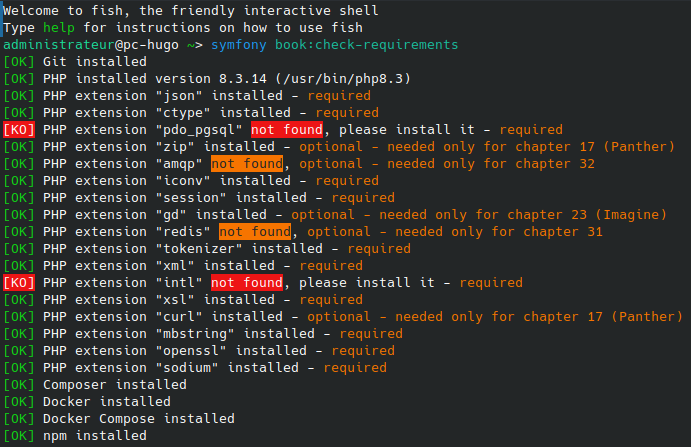
\includegraphics[scale=.6]{../images/book.png}
		\caption{\textit{Output} de la commande "symfony book:check-requirements" }
	\end{center}
\end{figure}	

\newpage
		Une fois cette vérification faite, nous pouvions passer à l'installation du projet. C'est Hugo L qui s'en est chargé. Il ne restait ensuite qu'à déposer le projet installé sur le dépôt GitHub, puis aux autres membres de cloner le dépôt sur leurs ordinateurs. Pour que les autres membres du groupe aient une configuration identique du projet, ils devaient procéder à des étapes supplémentaires : \\
		\begin{itemize}
			\item Installer Symfony avec la commande \textit{composer install}
			\item Créer le fichier \textit{.env.local}, car ce dernier n'était pas présent sur le dépôt, étant situé dans le fichier \textit{.gitignore} \\
		\end{itemize}
		
		Pour l'installation, nous avons suivi à la lettre la ressource de cours concernant l'installation de Symfony 6.4 avec le CLI. Il n'y a eu aucun problème durant cette installation.
		
		\subsection{Dépôt GitHub du projet}
		
		 \textbf{URL du dépôt GitHub du projet : \url{https://github.com/hugolgs-dev/UEL313-Groupe3-S4}} \\
		 
		 
		 Le dépôt GitHub est organisé de la même manière que la majorité des projets sous Symfony. Les répertoires importants sont :\\
		 
		 \begin{itemize}
		 	\item \textbf{src/} : C'est ici que se trouve la majorité du code source du projet, avec notamment les controllers et les entités ; 
		 	\item \textbf{templates/} : Ce répertoire regroupe tous les fichiers Twig, responsables du rendu des pages ; 
		 	\item \textbf{public/} : On y trouve les fichiers accessibles publiquement, depuis le site web : les fichiers CSS, JavaScript, ou encore les images. \\
		 \end{itemize} 
		 
		 
\begin{figure}[!h]
	\begin{center}
		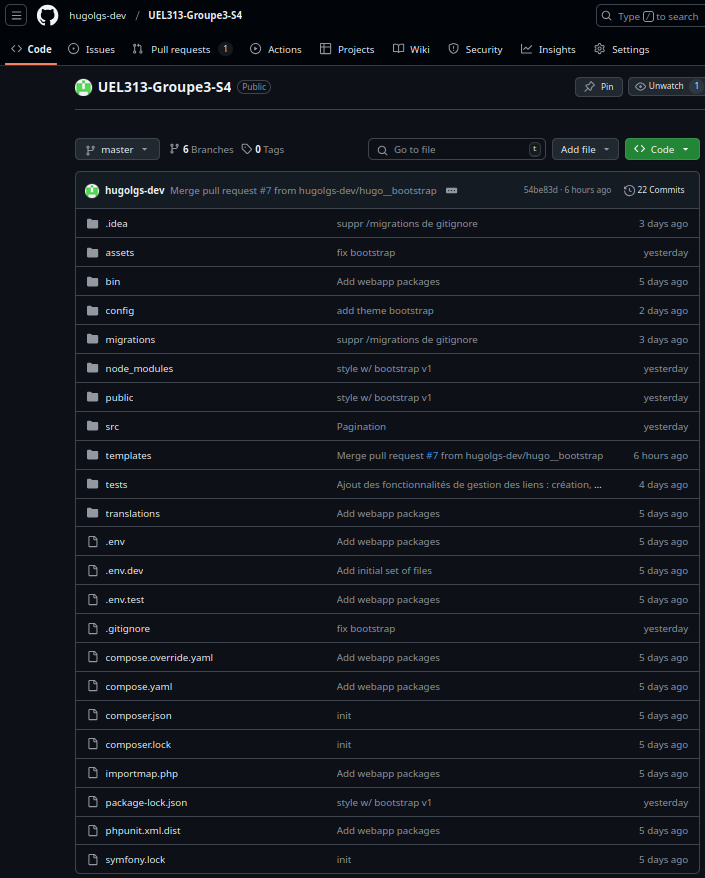
\includegraphics[scale=.6]{../images/depot.png}
		\caption{Dépôt GitHub du projet}
	\end{center}
\end{figure}	
			
\newpage
	\subsection{Création du CRUD}
	
	Dans un premier temps, nous avons mis en place l'entité \textit{Link.php}, grâce à Doctrine \cite{doctrine}, l'ORM de Symfony, et à la commande \textit{php bin/console make:entity}. Ensuite, nous avons appliqué les changements grâce aux migrations, en utilisant les commandes \textit{php bin/console make:migration} et \textit{php bin/console doctrine:migrations:migrate}. \\
	Une fois ces étapes passées, nous avons pu créer le CRUD, avec la commande \textit{php bin/console make:crud}, qui permet de générer son template et son controller. \\ 
	Après avoir apporté quelques finitions, le CRUD permettant de gérer des liens sur le site est entièrement opérationnel.
	
	\subsection{Problèmes migrations}

	Lors de la mise en place du CRUD, certains membres de l'équipe ont rencontré des erreurs en effectuant un \textit{git pull} pour récupérer les modifications sur la branche \textit{master}. Ces erreurs étaient dues à des conflits entre les migrations locales et celles présentes dans le dépôt. Par exemple, l'impossibilité de créer une nouvelle table "Links" ou un message indiquant que la "table article existe déjà". \\

	Pour résoudre ce problème, nous avons convenu de deux points essentiels : \\
	\begin{itemize}
		\item Ajouter les fichiers de migration au fichier \textit{.gitignore}.
		\item Supprimer les fichiers de migration déjà présents dans le dépôt. \\
	\end{itemize} 

	En appliquant ces bonnes pratiques, nous avons évité des conflits similaires à l'avenir.

	\subsection{Ajout de Bootstrap 5.3 au projet}
	
	Dans un premier temps, nous avions installé Bootstrap via le CDN. Cependant, les changements apportés sur le HTML avec Bootstrap n'étaient pas pris en compte, bien que les fichiers s'affichaient dans l'onglet "Réseau" de l'inspecteur du navigateur. \\

	Nous avons donc dû installer Bootstrap en téléchargeant l'archive .zip depuis le site web officiel \cite{bootstrap}. Ensuite, nous avons placé les dossiers \textit{css/} et \textit{js/} dans le répertoire \textit{public/} du site. Avec cette méthode, Bootstrap a fonctionné parfaitement. \\

\begin{figure}[!h]
	\begin{center}
		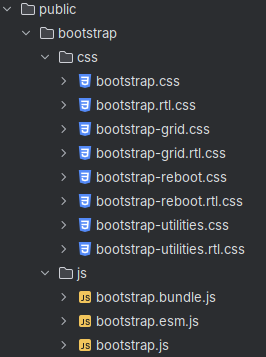
\includegraphics[scale=1]{../images/bootstrap.png}
		\caption{Répertoire public du site}
	\end{center}
\end{figure}

\newpage
		\subsubsection{Utilisation de Bootstrap}

	Pour ce projet, notre objectif était d'obtenir un visuel simple et épuré, particulièrement au niveau des formulaires. Nous voulions que l'expérience utilisateur soit la plus agréable possible.

\begin{figure}[!h]
	\begin{center}
		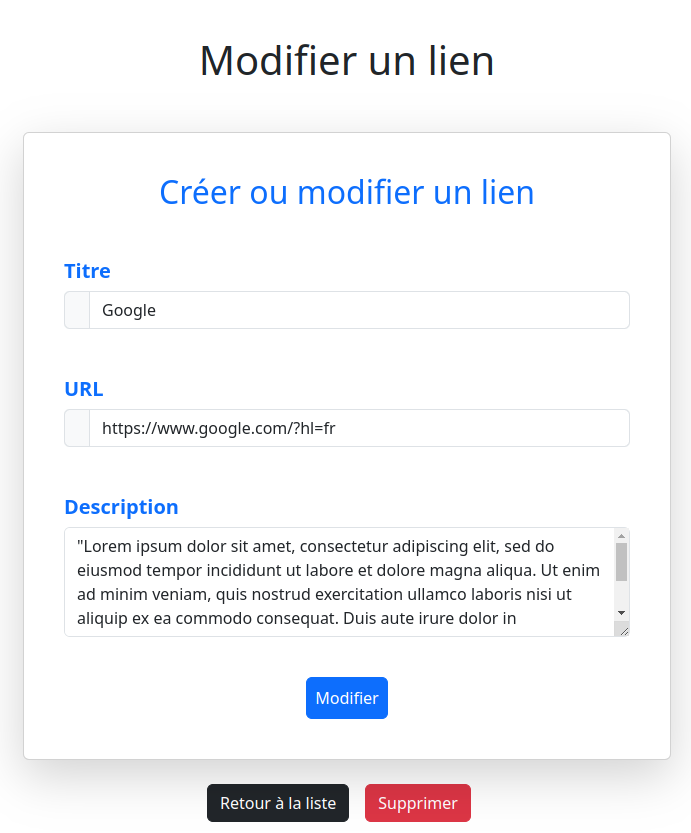
\includegraphics[scale=.6]{../images/forms.png}
		\caption{Formulaire épuré avec Bootstrap}
	\end{center}
\end{figure}

\newpage

\section{Conclusion}

Durant cette dernière semaine, nous avons appris à collaborer efficacement et à surmonter les défis techniques ensemble. Le choix de Symfony et l'organisation mise en place nous ont permis de mener à bien le projet tout en respectant les objectifs initiaux. \\


\printbibliography

\end{document}
